\section{Background}\label{sec:background}

\subsection{The Memory Hierarchy Review}\label{subsec:hierarchy}

Modern architectures take advantage of fast on-chip caches
to overcome the ``memory wall''.
As a compromise between direct mapped caches
and full-associative caches,
set-associative caches have been the dominant choice for real-world architectures.
To understand how cache sharing causes
inter-thread cache conflicts
and hurts GEMM performance, we review some details
about the working mechanism of set-associative caches and
the memory hierarchy of modern processors.

A set-associative cache can be defined by a 4-tuple $(c, l, n, nt)$,
in which $c$ is the cache capacity, $l$ is the cache line size,
$n$ is ways-of-associativity,
and $nt$ indicates the number of cores sharing the cache.
The whole cache memory is divided into $ns=c/l/n$ sets,
identified by indices in $\mathcal{S} = [0, ns)$,
with each set containing $n$ cache lines.
Generally, $ns$ is a power-of-two.
An indexing function $\varphi: \mathcal{A} \mapsto \mathcal{S}$ is responsible for
mapping addresses from the address space $\mathcal{A}$
(either virtual or physical) to the cache sets in
$\mathcal{S}$.
The data at $addr \in \mathcal{A}$ must be fetched
into the cache set $\varphi(addr) \in \mathcal{S}$ if requested.
A classic implementation of the indexing function is shown below,
%% $\varphi(addr) = (addr \gg log_2(l)) ~\&~ (ns-1)$,
with $\gg$ and $\&$ representing logical-shift-right and bitwise-and operations, respectively:
\begin{equation*}
  \varphi(addr) = (addr \gg log_2(l)) ~\&~ (ns-1)
  \label{eq:phi}
\end{equation*}
It is an extraction of the $log_2(ns)$ bits starting from the $log_2(l)$
position in $addr$'s binary form.

It is easy to prove that any continuous memory block
that is no larger than $c/n$
cannot conflict with itself.
We define a quantity, way-capacity, denoted as $wc=c/n$,
to represent this size bound for conflict-free memory blocks.

The main memory, $NL$ levels of caches, and $NT$ processor cores
forming a memory hierarchy are generally organized in terms
of an $NL+2$ level regular tree structure.
The processor cores at level $0$ are leaves,
the caches at levels $1$ -- $NL$ are intermediate nodes,
and the main memory at level $NL+1$ is the tree root.
Any node in the memory hierarchy can be identified by
its layer and its unique index at the layer $(layer, index)$.
The number of nodes at layer $l$ is $NT / nt_l$.

Throughout this paper, our example platform will be
a 4-core processor with
$NL=2$ levels of caches.
Figure~\ref{fig:hierarchy} shows its memory hierarchy 
and Table~\ref{tab:cluster} lists its
architectural parameters. 
Each core has 32 128-bit (16B) vector registers,
each capable of storing 2 double precision floating-point numbers.
For convenience, a processor core at level 0
is represented by its registers, which can be viewed as a special
level-0 cache $L0 = (512B, 16B, 32, 1)$ with programmable replacement policy.

\begin{figure}
  \centering
  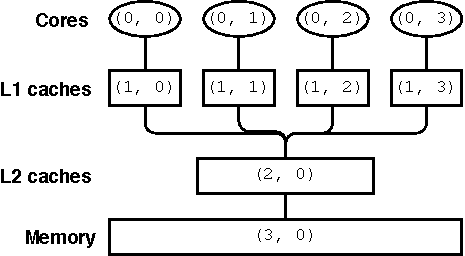
\includegraphics[width=.45\textwidth]{figures/cluster-new}
  \caption{Memory hierarchy of the 4-core processor
    (nodes labeled with $(layer,index)$)}
  \label{fig:hierarchy}
\end{figure}

\begin{table}
  \centering
  \caption{Architectural parameters of the 4-core processor}
  %% (see Section~\ref{subsec:hierarchy} for meanings of symbols in the header row)
  \label{tab:cluster}
  \begin{tabular}{lccccccl}
    \toprule
    Type & $c$ & $n$ & $l$ & $nt$ & $ns$ & $wc$ & Policy \\
    \midrule
    L0 Registers  & 512B & 32 & 16B & 1 & 1 & 16B & Programmable \\
    L1 Data    & 32KB & 2  & 64B & 1 & 256 & 16KB & LRU \\
    L2 Unified & 2MB  & 16 & 64B & 4 & 2048 & 128KB & Pseudo-Random \\
    \bottomrule
  \end{tabular}
\end{table}

\subsection{Structure of GEMM}\label{subsec:gemm}

GEMM performs a matrix-multiply-accumulate operation $C = \beta C + \alpha A B$,
where $A, B$ and $C$ are matrices of sizes
$M \times K$, $K \times N$ and $M \times N$, respectively,
and $\alpha$, $\beta$ are scalars.
While this operation is algorithmically simple,
so that a 3-deep loop nest suffices to accomplish it,
a high-performance implementation can be quite
sophisticated due to the presence of multi-level memory
hierarchy on modern processors.
Figure~\ref{fig:gemm} shows the structure of GEMM program from
the OpenBLAS library~\cite{openblas}.
Each loop (in the original 3-deep loop nest) is tiled,
resulting in a total of six loops (referred to as layers 1 -- 6).
%% Loop tiling, together with data packing and prefetching,
%% serves to improve data locality and overlap computation
%% and memory access effectively.

\begin{figure*}[t]
  \centering
  \includegraphics[width=\textwidth]{figures/gemm}
  \caption{Structure of blocked GEMM}
  \label{fig:gemm}
\end{figure*}

In this blocked algorithm, the loops over the $N$, $K$ and $M$
matrix dimensions are tiled by sizes $N_c$, $K_c$ and $M_c$ at 
layers 1, 2 and 3, respectively.
At layers 4 and 5, the $N$ and $M$ dimensions are further tiled by sizes
$N_r$ and $M_r$, respectively.
As a result, the innermost loop at layer 6 goes over the $K$
dimension for a total of $K_c$ times,
with each iteration performing a rank-1 update on
the $M_r \times N_r$ sub-matrix of $C$, as shown at layer 7.
In OpenBLAS, matrix $C$ is scaled by $\beta$ before the loops,
so the multiply-accumulate operation at layer 7 does not have to scale $C$ again.
Tiling factors $N_c$, $K_c$, $M_c$, $N_r$ and $M_r$ are carefully selected so that
matrices on each level fit into a certain level in the memory hierarchy.
Equations~(\ref{eq:constraints.reg}) -- (\ref{eq:constraints.l3}) express
the constraints on these tiling factors:
\begin{eqnarray}
  es (M_r + N_r + M_r N_r) & \le & c_{0} \label{eq:constraints.reg}\\
  nt_{1} \cdot es (N_r K_c + 2 M_r K_c) & \le & c_{1} \label{eq:constraints.l1}\\
  nt_{2} \cdot es (M_c K_c + 2 N_r K_c) & \le & c_{2} \label{eq:constraints.l2}\\
  es (N_c K_c + nt_{3} \cdot M_c K_c)   & \le & c_{3} \label{eq:constraints.l3}
\end{eqnarray}
Here, $es$ denotes the size of a matrix element,
e.g., 8B for a double precision floating-point number,
and $c_l$ denotes the capacity of the register file or cache at level $l$.
By (\ref{eq:constraints.reg}), $M_r$ and $N_r$ are so
constrained that $M_r$ elements from $A$,
$N_r$ elements from $B$ and $M_r \times N_r$ elements from $C$ can
fit into the registers (the pseudo level-0 cache).
By (\ref{eq:constraints.l1}), $K_c$ is so constrained that $B_4$ ($N_r \times K_c$),
$A_4$ ($M_r \times K_c$), and $A_4$'s counterpart in the next iteration
at layer 5 fit into the L1 cache.
By (\ref{eq:constraints.l2}), $M_c$ is so constrained that $A_3$ ($M_c \times K_c$),
$B_3$ ($N_r \times K_c$), and $B_3$'s counterpart in the next iteration
at layer 4 fit into the L2 cache.
Finally, by (\ref{eq:constraints.l3}), $N_c$ is so constrained that 
$B_2$ ($K_c \times N_c$) and $A_2$ ($M_c \times K_c$) fit into the L3 cache.
Larger matrices at higher layers 1 -- 3 always reside in main memory.

\begin{comment}
Table~\ref{tab:factors} shows the procedure choosing various tiling factors.
In each row, one or more tiling factors (column 1) is determined
by a size constraint (column 3) related to a certain level
in the memory hierarchy (column 2).
\begin{table}
  \centering
  \caption{Procedure of choosing tiling factors}
  \label{tab:factors}
  \begin{tabular}{cccl}
    \toprule
    factor & memory & constraint \\
    \midrule
    $M_r$, $N_r$ & registers & $M_r + N_r + M_r N_r \le Regs$ \\
    $K_c$        & L1 cache  & $N_r K_c + 2 M_r K_c \le L1$ \\
    $M_c$        & L2 cache  & $M_c K_c + 2 N_r K_c \le L2$ \\
    $N_c$        & L3 cache  & $N_c K_c + M_c K_c \le L3$ \\
    \bottomrule
  \end{tabular}
\end{table}
\end{comment}

Goto~\cite{gotogemm} factors out the innermost three loops at layers 4 -- 6 for
computing $C_2\ = C_2 + \alpha A_2 B_2$ as an architecture-dependent kernel,
known as  GEBP (GEneral multiply of a Block of $A$ and a Panel of $B$).
It is worthy noting that before GEBP is called (at layer 3),
$A_1[ii:ii+M_c-1][:]$ and $B_1$ are packed into $A_2$ and $B_2$
in a special continuous layout,
so consecutive memory access is ensured within the GEBP kernel.
GotoBLAS~\cite{gotoblas}, and its successor, OpenBLAS~\cite{openblas},
implement GEMM programs based on this factorization,
with GEBP highly optimized for the target processor (often coded in assembly).

As stated in Section~\ref{sec:intro}, a GEMM implementation
is made up by a kernel routine and an overall workload-partitioning strategy.
In Figure~\ref{fig:gemm}, GEBP serves as the kernel routine,
and the overall workload-partitioning strategy is defined by the three outer loops at layers 1 -- 3.
Developers can decide how to partition the workload by choosing
tile factors $M_c$, $N_c$ and $K_c$,
and how to schedule GEBP tasks by interchanging loop orders at layers 1 - 3.
Either the $jj$ loop at layer 1 or the $ii$ loop at layer 3, or both,
can be parallelized in a multi-threaded context.
Specifically, the implementation in Figure~\ref{fig:gemm}
chooses an $jj\textrm{-}kk\textrm{-}ii$ loop order
and parallelizes the $ii$ loop at layer 3.
Different threads work on different parts of $A_1$
and share the same $B_1$.

As a result, there are multiple $A_2$ instances (one per thread)
and a single $B_2$ instance (shared by all threads).
To understand how the $ii$ loop at layer 3 is parallelized on the 4-core processor, 
Figure.~\ref{fig:workload} shows the data accessing patterns
of a single thread $T_1$.
While all color shaded submatrices are accessed by $T_1$,
only the z-curve masked submatrices (a subset of color shaded ones)
are packed by the thread.
In other words, each thread packs its own $A_2$ instance and  all the threads collaboratively pack the unique $B_2$ instance.
%% We will use the OpenBLAS GEMM implementation in Figure.~\ref{fig:gemm}
%% in discussion and evaluation throughout the paper.

\begin{figure}[t]
  \centering
  \includegraphics[width=.4\textwidth]{figures/workload}
  \caption{GEMM parallelization with 4 threads and data accessing patterns of thread $T_1$}
  \label{fig:workload}
\end{figure}

\subsection{Cache Conflicts in GEMM}\label{subsec:cache-conflicts}

For set-associative caches, cache misses can be categorized
into capacity and conflict misses.
While the constraints (\ref{eq:constraints.reg}) -- (\ref{eq:constraints.l3})
aim to avoid capacity misses,
conflict misses cannot be eliminated completely.
%% We use the term ``cache conflict'' to represent conflict miss events.

In Figure.~\ref{fig:gemm}, the packed matrix $A_2$
will be read $N_c/N_r$ times within a single GEBP execution,
and is expected to reside in the 
L2 cache during all $N_c/N_r$ iterations at layer 4.
The packed matrix $B_4$ is similar in that it is expected to
reside in the L1 cache during all $M_c/M_r$ iterations at layer 5.
In general, even with carefully selected tile factors,
matrix data can still be evicted.
For example, some data structures other than the packed matrices
or program code (in case of a unified cache) may be fetched into the
cache set where the matrix data reside in.
Such cache conflicts are referred to as
intra-thread cache conflicts
because it occurs within the execution of a single thread.
To deal with intra-thread conflicts,
the GEBP kernel repeatedly prefetch data from $A_4$ and $B_4$ to the L1 cache
in every iteration at layer 6 before it actually reads them in case of
the data being evicted accidentally.
As GEBP accesses the matrix data much more frequently than other
data structures, this repeated prefetching strategy
can reduce the penalty caused by intra-thread conflicts.

In contrary to intra-thread cache conflicts,
there exists another kind of cache conflicts, called
inter-thread cache conflicts, on architectures with shared caches.
Suppose two working threads, $T_0$ and $T_1$, are running independently
on the 4-core processor in Figure.~\ref{fig:hierarchy}
to accomplish a GEMM operation.
At time $t_s$, $T_0$ prefetches some data at address $addr_0$
to cache set $\varphi_2(addr_0)$ of the shared L2 cache.
The data will be actually read at time $t_e$.
Then at some time $t_m$ ($t_s < t_m < t_e$),
$T_1$ prefetches data at address $addr_1$ to the L2 cache.
If $\varphi_2(addr_1)=\varphi_2(addr_0)$, then the
data at $addr_1$ and $addr_0$ will be fetched into the same cache set.
As the shared L2 cache has a non-LRU policy,
the data at $addr_0$ may suffer an eviction before it is actually read,
i.e., a conflict miss occurs.

In GEMM, every cache is utilized aggressively
so that almost all its cache space is expected to be occupied by packed matrices.
Prefetch instructions from different threads are executed repeatedly,
interleaved in an unpredictable manner.
So inter-thread cache conflicts described above
can occur frequently on non-LRU shared caches,
thus making the technique dealing with intra-thread cache conflicts ineffective.
The situation worsens with more threads sharing the same cache.

